\subsection{MilNet architecture}
Multi-Instance Learning Networks were introduced in \cite{angelidis2017multiple} as a tool for predicting segment sentiment labels when having only document sentiment labels as a ground truth. In our setting, sentences are treated as segments, and comments --- as documents. \\
The process of training a MilNet can be described with the following steps (see Figure \ref{milnet}):
\begin{enumerate}[label=(\alph*)]
    \item Split each document in the dataset into segments;
    \item Compute segment embeddings as a convolution of corresponding word embeddings;
    \item Compute segment labels using a recurrent neural network with gated recurrent units;
    \item Compute document label using attention mechanism;
    \item Do backpropagation with respect to ground truth of {\bf document} labels only.
\end{enumerate}

\begin{figure}[h]
\centerline{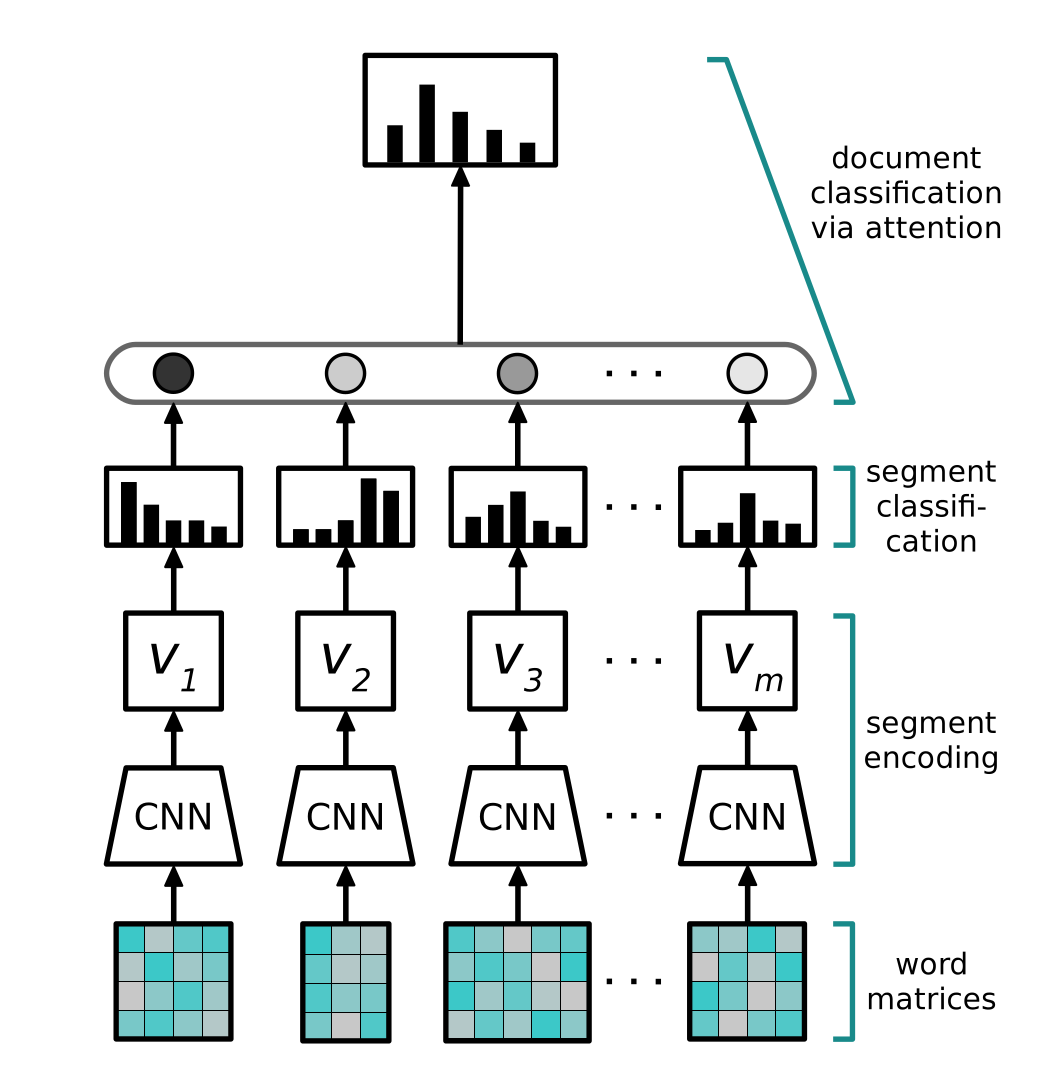
\includegraphics[scale=.2]{images/milnet.png}}
\caption{MilNet architecture.}
\label{milnet}
\end{figure}
After the training, one can extract segment sentiments by ignoring the last two steps. \\
For this project, we were interested in exploring the potential of BERT embeddings in such architecture. For this, we skipped the first two steps by using precomputed segment embeddings. 

\subsection{Embeddings}

\subsubsection{Vector semantics embeddings}
Words that occur in similar contexts tend to have similar meanings. The concept of vector semantics instantiates this linguistic hypothesis by learning representations of the meaning of words, called {\bf embeddings}, directly from their distributions in texts. These representations are used in every natural language processing application that makes use of meaning \cite{jurafskyBook}.

\subsubsection{Feature representation for neural networks}
We can think of a feed-forward neural network as a function $NN(x)$ that takes as input a $d_{in}$ dimensional vector $x$ and produces a $d_{out}$ dimensional output vector. When dealing with natural language, the input $x$ encodes features  such  as  words, part-of-speech tags or other linguistic information. Perhaps the biggest conceptual jump when moving from sparse-input linear models to neural-network based models is to stop representing each feature as a unique dimension (the so called one-hot representation) and representing them instead as dense vectors called {\bf embeddings}. That is, each core feature is embedded into a $d$ dimensional space, and represented as a vector in that space \cite{goldberg2015primer}.

\subsubsection{Contextualized Embeddings}
With traditional embeddings such as {\bf GloVe} and {\bf Word2Vec}, each word in a vocabulary gets its own representation, independent of the context on which they are used. Even though this may be useful for many problems, it is logical to think that the semantic information of a word depends on the context in which it is used. For example, consider the word "jaguar", which can have different word senses depending on the context: an animal, a car or a guitar.\\
%An example of this is the word "jaguar", which can have different word senses depending on the context: an animal, a car or a guitar.\\
Even when using the same word sense of a word, there may be semantic differences dependent on the context in which the word is used. Contextual embeddings like {\bf ELMo} and {\bf BERT} address this issue by giving each token of a sentence its own embedding depending on the entire context of the sentence.

\subsubsection{Sentence Embeddings}
Sentence embeddings are dense vectors that summarize different properties of a sentence (e.g. its meaning), thereby extending the very popular concept of word embeddings. In contrast to task-specific representations, such as the ones trained specifically for tasks like textual entailment or sentiment, such sentence embeddings are trained in a task-agnostic manner on large datasets. As a consequence, they often perform better when little labeled data is available \cite{rckl2018concatenated}.

\subsubsection{Transfer learning and model pretraining}
Language  model  pretraining  has  been  shown  to be effective for improving many natural language processing tasks \cite{devlin2018bert}. This model pretraining consists in training a neural network in one task (usually language modeling), and then using the intermediate representation of a deep layer of the network as embeddings for another model. Such approach allows to transfer the syntactic and semantic properties learned by the language modeling model to other models that focus on different tasks.\\
There  are  two  existing  strategies  for  applying pretrained language representations to downstream tasks: feature-based and fine-tuning. The feature-based  approach, such as {\bf ELMo}, uses task-specific architectures that include the pretrained representations as additional features. The fine-tuning approach, such as the Generative pretrained Transformer ({\bf OpenAIGPT}), introduces minimal task-specific  parameters,  and  is  trained  on  the downstream  tasks  by  simply  fine-tuning all pretrained parameters.

\subsubsection{BERT: Bidirectional Encoder Representations from Transformers}
{\bf BERT} improves the fine-tuning based approaches by using a “masked language  model” (MLM)  pretraining  objective. The masked language model randomly masks some of the tokens from the input, and the objective is to predict the original vocabulary id of the masked word  based only on its context \cite{devlin2018bert}.

\subsubsection{RoBERTa}
RoBERTa is an improved recipe for training BERT models, that can match or exceed the performance of all of the post-BERT methods. It includes modifications to BERT such as: (1) training the model longer, with bigger batches, over more data; (2) removing the next sentence prediction objective; (3) training on longer sequences; and (4) dynamically changing the masking pattern applied to the training data \cite{liu2019roberta}.

\subsubsection{XLING}
XLING generalizes  the  concept  of  average  word  embeddings to power mean word embeddings. In this method, instead of using the component-wise arithmetic averages of the word embeddings to generate sentence embeddings, the concateniation of the so-called power means is used \cite{rckl2018concatenated}.
